\chapter{Cheating with \\ Feature Subset Selection}
\label{ch:fss-overfitting}

\marginnote{\textbf{\textsf{We will borrow a gene expression data set from Gene Expression Omnibus for our example. There is a particular widget in the Orange bioinformatics add-on that we could use to fetch this and similar data sets. Instead, we will rely on the GEO data set gds360 available at \url{http://file.biolab.si/datasets/gds360.pkl}.}}}
%
Consider a typical gene expression data set with samples in rows and genes expressions in columns. These data sets are usually fat; they include more genes than samples. Fat data sets are almost typical for systems biology. When we label the samples with phenotype, and our task is phenotype classification, many features (genes) will be irrelevant. Most often, only a few features correlate with class. So why not simply select a set of most informative features first and then do the whole analysis? At least cross-validation will then work much faster, as the model inference algorithms will deal with much smaller data tables. Cool. What a nice trick! Let’s try it out in the following workflow.

\begin{figure}[h]
    \centering
    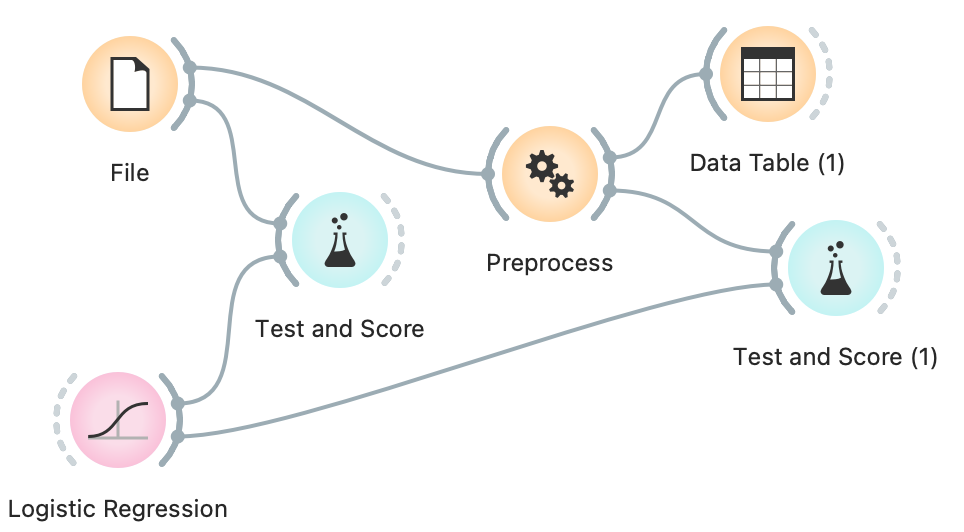
\includegraphics[scale=0.5]{fss-overfitting-workflow.png}
    \caption{$\;$}
\end{figure}

% \begin{marginfigure}
%     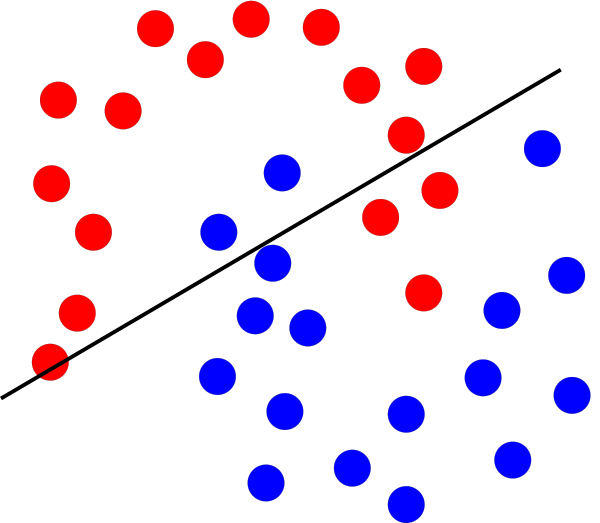
\includegraphics[width=50mm]{linear-regression.png}%
%     \caption{Decision boundary of a linear regression classifier.}
% \end{marginfigure}

The workflow above uses the data preprocessing widget, which we have configured to select the five most informative features.

\begin{figure}[h]
    \centering
    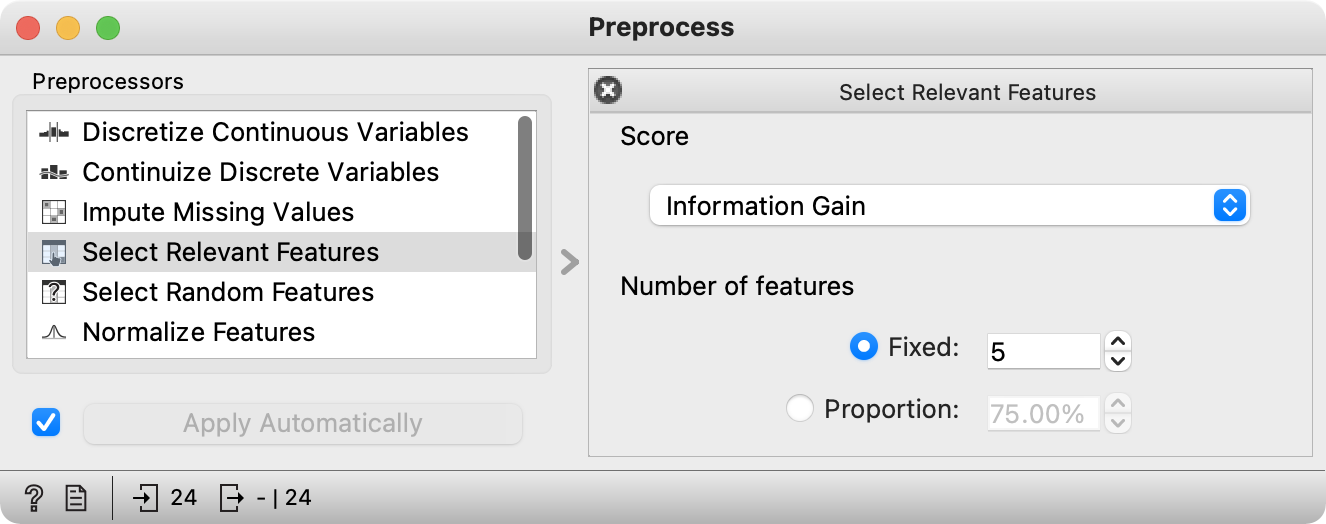
\includegraphics[scale=0.4]{preprocess.png}
    \caption{$\;$}
\end{figure}

Observe the classification accuracy obtained on the original data set and the data set with the five best-selected features. What is happening? What is there such difference in classification accuracy?